
%% bare_conf_compsoc.tex
%% V1.4b
%% 2015/08/26
%% by Michael Shell
%% See:
%% http://www.michaelshell.org/
%% for current contact information.
%%
%% This is a skeleton file demonstrating the use of IEEEtran.cls
%% (requires IEEEtran.cls version 1.8b or later) with an IEEE Computer
%% Society conference paper.
%%
%% Support sites:
%% http://www.michaelshell.org/tex/ieeetran/
%% http://www.ctan.org/pkg/ieeetran
%% and
%% http://www.ieee.org/

%%*************************************************************************
%% Legal Notice:
%% This code is offered as-is without any warranty either expressed or
%% implied; without even the implied warranty of MERCHANTABILITY or
%% FITNESS FOR A PARTICULAR PURPOSE! 
%% User assumes all risk.
%% In no event shall the IEEE or any contributor to this code be liable for
%% any damages or losses, including, but not limited to, incidental,
%% consequential, or any other damages, resulting from the use or misuse
%% of any information contained here.
%%
%% All comments are the opinions of their respective authors and are not
%% necessarily endorsed by the IEEE.
%%
%% This work is distributed under the LaTeX Project Public License (LPPL)
%% ( http://www.latex-project.org/ ) version 1.3, and may be freely used,
%% distributed and modified. A copy of the LPPL, version 1.3, is included
%% in the base LaTeX documentation of all distributions of LaTeX released
%% 2003/12/01 or later.
%% Retain all contribution notices and credits.
%% ** Modified files should be clearly indicated as such, including  **
%% ** renaming them and changing author support contact information. **
%%*************************************************************************


% *** Authors should verify (and, if needed, correct) their LaTeX system  ***
% *** with the testflow diagnostic prior to trusting their LaTeX platform ***
% *** with production work. The IEEE's font choices and paper sizes can   ***
% *** trigger bugs that do not appear when using other class files.       ***                          ***
% The testflow support page is at:
% http://www.michaelshell.org/tex/testflow/



\documentclass[conference,compsoc]{IEEEtran}
% Some/most Computer Society conferences require the compsoc mode option,
% but others may want the standard conference format.
%
% If IEEEtran.cls has not been installed into the LaTeX system files,
% manually specify the path to it like:
% \documentclass[conference,compsoc]{../sty/IEEEtran}





% Some very useful LaTeX packages include:
% (uncomment the ones you want to load)


% *** MISC UTILITY PACKAGES ***
%
%\usepackage{ifpdf}
% Heiko Oberdiek's ifpdf.sty is very useful if you need conditional
% compilation based on whether the output is pdf or dvi.
% usage:
% \ifpdf
%   % pdf code
% \else
%   % dvi code
% \fi
% The latest version of ifpdf.sty can be obtained from:
% http://www.ctan.org/pkg/ifpdf
% Also, note that IEEEtran.cls V1.7 and later provides a builtin
% \ifCLASSINFOpdf conditional that works the same way.
% When switching from latex to pdflatex and vice-versa, the compiler may
% have to be run twice to clear warning/error messages.



\usepackage{hyperref}



% *** CITATION PACKAGES ***
%
\ifCLASSOPTIONcompsoc
  % IEEE Computer Society needs nocompress option
  % requires cite.sty v4.0 or later (November 2003)
  \usepackage[nocompress]{cite}
\else
  % normal IEEE
  \usepackage{cite}
\fi
% cite.sty was written by Donald Arseneau
% V1.6 and later of IEEEtran pre-defines the format of the cite.sty package
% \cite{} output to follow that of the IEEE. Loading the cite package will
% result in citation numbers being automatically sorted and properly
% "compressed/ranged". e.g., [1], [9], [2], [7], [5], [6] without using
% cite.sty will become [1], [2], [5]--[7], [9] using cite.sty. cite.sty's
% \cite will automatically add leading space, if needed. Use cite.sty's
% noadjust option (cite.sty V3.8 and later) if you want to turn this off
% such as if a citation ever needs to be enclosed in parenthesis.
% cite.sty is already installed on most LaTeX systems. Be sure and use
% version 5.0 (2009-03-20) and later if using hyperref.sty.
% The latest version can be obtained at:
% http://www.ctan.org/pkg/cite
% The documentation is contained in the cite.sty file itself.
%
% Note that some packages require special options to format as the Computer
% Society requires. In particular, Computer Society  papers do not use
% compressed citation ranges as is done in typical IEEE papers
% (e.g., [1]-[4]). Instead, they list every citation separately in order
% (e.g., [1], [2], [3], [4]). To get the latter we need to load the cite
% package with the nocompress option which is supported by cite.sty v4.0
% and later.





% *** GRAPHICS RELATED PACKAGES ***
%
\ifCLASSINFOpdf
  \usepackage[pdftex]{graphicx}
  % declare the path(s) where your graphic files are
  % \graphicspath{{../pdf/}{../jpeg/}}
  % and their extensions so you won't have to specify these with
  % every instance of \includegraphics
  % \DeclareGraphicsExtensions{.pdf,.jpeg,.png}
\else
  % or other class option (dvipsone, dvipdf, if not using dvips). graphicx
  % will default to the driver specified in the system graphics.cfg if no
  % driver is specified.
  % \usepackage[dvips]{graphicx}
  % declare the path(s) where your graphic files are
  % \graphicspath{{../eps/}}
  % and their extensions so you won't have to specify these with
  % every instance of \includegraphics
  % \DeclareGraphicsExtensions{.eps}
\fi
% graphicx was written by David Carlisle and Sebastian Rahtz. It is
% required if you want graphics, photos, etc. graphicx.sty is already
% installed on most LaTeX systems. The latest version and documentation
% can be obtained at: 
% http://www.ctan.org/pkg/graphicx
% Another good source of documentation is "Using Imported Graphics in
% LaTeX2e" by Keith Reckdahl which can be found at:
% http://www.ctan.org/pkg/epslatex
%
% latex, and pdflatex in dvi mode, support graphics in encapsulated
% postscript (.eps) format. pdflatex in pdf mode supports graphics
% in .pdf, .jpeg, .png and .mps (metapost) formats. Users should ensure
% that all non-photo figures use a vector format (.eps, .pdf, .mps) and
% not a bitmapped formats (.jpeg, .png). The IEEE frowns on bitmapped formats
% which can result in "jaggedy"/blurry rendering of lines and letters as
% well as large increases in file sizes.
%
% You can find documentation about the pdfTeX application at:
% http://www.tug.org/applications/pdftex





% *** MATH PACKAGES ***
%

\usepackage{amsmath}
\usepackage{amssymb}
% A popular package from the American Mathematical Society that provides
% many useful and powerful commands for dealing with mathematics.
%
% Note that the amsmath package sets \interdisplaylinepenalty to 10000
% thus preventing page breaks from occurring within multiline equations. Use:
%\interdisplaylinepenalty=2500
% after loading amsmath to restore such page breaks as IEEEtran.cls normally
% does. amsmath.sty is already installed on most LaTeX systems. The latest
% version and documentation can be obtained at:
% http://www.ctan.org/pkg/amsmath





% *** SPECIALIZED LIST PACKAGES ***
%
\usepackage{algorithmicx}
\usepackage{algpseudocode}
% algorithmic.sty was written by Peter Williams and Rogerio Brito.
% This package provides an algorithmic environment fo describing algorithms.
% You can use the algorithmic environment in-text or within a figure
% environment to provide for a floating algorithm. Do NOT use the algorithm
% floating environment provided by algorithm.sty (by the same authors) or
% algorithm2e.sty (by Christophe Fiorio) as the IEEE does not use dedicated
% algorithm float types and packages that provide these will not provide
% correct IEEE style captions. The latest version and documentation of
% algorithmic.sty can be obtained at:
% http://www.ctan.org/pkg/algorithms
% Also of interest may be the (relatively newer and more customizable)
% algorithmicx.sty package by Szasz Janos:
% http://www.ctan.org/pkg/algorithmicx




% *** ALIGNMENT PACKAGES ***
%
\usepackage{array}
% Frank Mittelbach's and David Carlisle's array.sty patches and improves
% the standard LaTeX2e array and tabular environments to provide better
% appearance and additional user controls. As the default LaTeX2e table
% generation code is lacking to the point of almost being broken with
% respect to the quality of the end results, all users are strongly
% advised to use an enhanced (at the very least that provided by array.sty)
% set of table tools. array.sty is already installed on most systems. The
% latest version and documentation can be obtained at:
% http://www.ctan.org/pkg/array


% IEEEtran contains the IEEEeqnarray family of commands that can be used to
% generate multiline equations as well as matrices, tables, etc., of high
% quality.




% *** SUBFIGURE PACKAGES ***
%\ifCLASSOPTIONcompsoc
%  \usepackage[caption=false,font=footnotesize,labelfont=sf,textfont=sf]{subfig}
%\else
%  \usepackage[caption=false,font=footnotesize]{subfig}
%\fi
% subfig.sty, written by Steven Douglas Cochran, is the modern replacement
% for subfigure.sty, the latter of which is no longer maintained and is
% incompatible with some LaTeX packages including fixltx2e. However,
% subfig.sty requires and automatically loads Axel Sommerfeldt's caption.sty
% which will override IEEEtran.cls' handling of captions and this will result
% in non-IEEE style figure/table captions. To prevent this problem, be sure
% and invoke subfig.sty's "caption=false" package option (available since
% subfig.sty version 1.3, 2005/06/28) as this is will preserve IEEEtran.cls
% handling of captions.
% Note that the Computer Society format requires a sans serif font rather
% than the serif font used in traditional IEEE formatting and thus the need
% to invoke different subfig.sty package options depending on whether
% compsoc mode has been enabled.
%
% The latest version and documentation of subfig.sty can be obtained at:
% http://www.ctan.org/pkg/subfig




% *** FLOAT PACKAGES ***
%
%\usepackage{fixltx2e}
% fixltx2e, the successor to the earlier fix2col.sty, was written by
% Frank Mittelbach and David Carlisle. This package corrects a few problems
% in the LaTeX2e kernel, the most notable of which is that in current
% LaTeX2e releases, the ordering of single and double column floats is not
% guaranteed to be preserved. Thus, an unpatched LaTeX2e can allow a
% single column figure to be placed prior to an earlier double column
% figure.
% Be aware that LaTeX2e kernels dated 2015 and later have fixltx2e.sty's
% corrections already built into the system in which case a warning will
% be issued if an attempt is made to load fixltx2e.sty as it is no longer
% needed.
% The latest version and documentation can be found at:
% http://www.ctan.org/pkg/fixltx2e


%\usepackage{stfloats}
% stfloats.sty was written by Sigitas Tolusis. This package gives LaTeX2e
% the ability to do double column floats at the bottom of the page as well
% as the top. (e.g., "\begin{figure*}[!b]" is not normally possible in
% LaTeX2e). It also provides a command:
%\fnbelowfloat
% to enable the placement of footnotes below bottom floats (the standard
% LaTeX2e kernel puts them above bottom floats). This is an invasive package
% which rewrites many portions of the LaTeX2e float routines. It may not work
% with other packages that modify the LaTeX2e float routines. The latest
% version and documentation can be obtained at:
% http://www.ctan.org/pkg/stfloats
% Do not use the stfloats baselinefloat ability as the IEEE does not allow
% \baselineskip to stretch. Authors submitting work to the IEEE should note
% that the IEEE rarely uses double column equations and that authors should try
% to avoid such use. Do not be tempted to use the cuted.sty or midfloat.sty
% packages (also by Sigitas Tolusis) as the IEEE does not format its papers in
% such ways.
% Do not attempt to use stfloats with fixltx2e as they are incompatible.
% Instead, use Morten Hogholm'a dblfloatfix which combines the features
% of both fixltx2e and stfloats:
%
% \usepackage{dblfloatfix}
% The latest version can be found at:
% http://www.ctan.org/pkg/dblfloatfix




% *** PDF, URL AND HYPERLINK PACKAGES ***
%
%\usepackage{url}
% url.sty was written by Donald Arseneau. It provides better support for
% handling and breaking URLs. url.sty is already installed on most LaTeX
% systems. The latest version and documentation can be obtained at:
% http://www.ctan.org/pkg/url
% Basically, \url{my_url_here}.




% *** Do not adjust lengths that control margins, column widths, etc. ***
% *** Do not use packages that alter fonts (such as pslatex).         ***
% There should be no need to do such things with IEEEtran.cls V1.6 and later.
% (Unless specifically asked to do so by the journal or conference you plan
% to submit to, of course. )
\usepackage{enumitem}
\usepackage[margin=0.5in]{geometry}

% correct bad hyphenation here
\hyphenation{op-tical net-works semi-conduc-tor}


\begin{document}
%
% paper title
% Titles are generally capitalized except for words such as a, an, and, as,
% at, but, by, for, in, nor, of, on, or, the, to and up, which are usually
% not capitalized unless they are the first or last word of the title.
% Linebreaks \\ can be used within to get better formatting as desired.
% Do not put math or special symbols in the title.
\title{Automatic Hilghter of Lengthy Legal Documents}


% author names and affiliations
% use a multiple column layout for up to three different
% affiliations
\author{\IEEEauthorblockN{Yanshu Hong}
\IEEEauthorblockA{Computer Science Department\\
Email: yanshuh@stanford.edu}
\and
\IEEEauthorblockN{Tian Zhao}
\IEEEauthorblockA{Electrical Engineering Department\\
Email: tianzhao@stanford.edu}}

% conference papers do not typically use \thanks and this command
% is locked out in conference mode. If really needed, such as for
% the acknowledgment of grants, issue a \IEEEoverridecommandlockouts
% after \documentclass

% for over three affiliations, or if they all won't fit within the width
% of the page (and note that there is less available width in this regard for
% compsoc conferences compared to traditional conferences), use this
% alternative format:
% 
%\author{\IEEEauthorblockN{Michael Shell\IEEEauthorrefmark{1},
%Homer Simpson\IEEEauthorrefmark{2},
%James Kirk\IEEEauthorrefmark{3}, 
%Montgomery Scott\IEEEauthorrefmark{3} and
%Eldon Tyrell\IEEEauthorrefmark{4}}
%\IEEEauthorblockA{\IEEEauthorrefmark{1}School of Electrical and Computer Engineering\\
%Georgia Institute of Technology,
%Atlanta, Georgia 30332--0250\\ Email: see http://www.michaelshell.org/contact.html}
%\IEEEauthorblockA{\IEEEauthorrefmark{2}Twentieth Century Fox, Springfield, USA\\
%Email: homer@thesimpsons.com}
%\IEEEauthorblockA{\IEEEauthorrefmark{3}Starfleet Academy, San Francisco, California 96678-2391\\
%Telephone: (800) 555--1212, Fax: (888) 555--1212}
%\IEEEauthorblockA{\IEEEauthorrefmark{4}Tyrell Inc., 123 Replicant Street, Los Angeles, California 90210--4321}}




% use for special paper notices
%\IEEEspecialpapernotice{(Invited Paper)}




% make the title area
\maketitle

% As a general rule, do not put math, special symbols or citations
% in the abstract
% \begin{abstract}
%   Lengthy legal documents are hard to read. In this paper, we propose a set of solutions that auto-highlights sentences 
%   which require special attention in a legal document. In the first section, we will talk about why it is important to 
%   have an auto-highlighter for reading legal documents. In the second section, we will give an overview of related works. In the
%   third section, we will summarize our methods of preprocessing data to build our corpus for training. Our major method is an 
%   application of Latent Dirichilet Allocation (LDA) model. In the fourth section, 
%   we will discuss our algorithms of detecting special sentences in a document, namely, by evaluting Local Outlier Factor (LOF) for 
%   each sentence and by using Agglomerative clustering. In the fifth section, we will discuss our methodologies of tuning the 
%   hyperparameters, e.g. number of intial clusters, number of topics in the LDA model. In the last section, we will discuss about
%   possible improvements.  
% \end{abstract}

% no keywords


% For peer review papers, you can put extra information on the cover
% page as needed:
% \ifCLASSOPTIONpeerreview
% \begin{center} \bfseries EDICS Category: 3-BBND \end{center}
% \fi
%
% For peerreview papers, this IEEEtran command inserts a page break and
% creates the second title. It will be ignored for other modes.
\IEEEpeerreviewmaketitle



\section{Introduction}
% no \IEEEPARstart
    Legal documents are known for being lengthy. To our knowledge, some categories of legal documents contain duplicated 
    information that do not require our attention. However, manually extracting non-duplicate information from documents requires
    considerable amount of effort. Thus, we want to use machine learning algorithms to pick up unordinary sentences for us.
    In this paper, we propose a set of algorithms that filters out duplicate information and 
    returns useful information to the user. We are able to train a learner that can mark unordinary parts of a legal 
    document for manual scrutinization. 

    Our learning process contains two phases. At the first phase, we pick some legal documents that contain common patterns, e.g. software user agreements, to form a knowledge base for the trainer. We then run \emph{LDA} \cite{lda} model on these documents. The \emph{LDA} model will return us with a set of common topics across the knowledge base.  

    At the second phase, we take a new piece of legal document as the test sample. We first remove common topic words from the test document to increase differences between sentences. We then use \emph{Word2Vec} \cite{one,two} to convert sentences into vectors. After generating the feature space, we run \emph{Agglomerative Clustering} and \emph{Local Outlier Factor(LOF)} \cite{lof} algorithms on the feature vectors to detect special sentences in the given document. Last, we use \emph{PCA} and \emph{t-SNE} to visualize our result. 

    % At the first learning phase, we pick some legal documents that contain common patterns, e.g. software user agreements, to 
    % form a knowledge base for our trainer. We then use \emph{LDA} \cite{lda} model to generate a set of common topics across the knowledge base. % TODO

    % At the second learning phase, our input is a new piece of legal document in the format of plain text. We first remove common topic words from our test document to increase the differences between sentences in the test document. We then use \emph{Word2Vec} \cite{one,two} to convert sentences into vectors. We then use \emph{Agglomerative Clustering} and \emph{Local Outlier Factor(LOF))} \cite{lof} algorithms to detect special sentences in the given document. Last, we use \emph{PCA} and \emph{t-SNE} to visualize our result. 

\section{Related Work}
  Though text-mining related works are often seen, few of them address the issue of sentence-level anormaly detection. However, we are able to draw inspirations from previous works on unsupervised auto-generation of document summary. 

  Qazvinian and Radev (2008) \cite{reviewcite1} presented two sentences selection models based on clusters generated by hierarchical clustering algorithms. \emph{C-RR} finds the largest cluster and rank the importance of sentences by their order of appearance in the cluster. \emph{C-lexrank} selects the most centered sentences within the cluster to be the salient ones. While their clustering strategy performs well on segmenting an article, their strategy on finding the salient sentences does not apply to our case. Based on their design, a sentence with the most common pattern would be chosen as a salient one. However, it is also the case that such sentence would contain the most duplicate information; therefore it should not require much attention from the reader.  

  Similarly, Nanba and Okumura (1999) \cite{reviewcite3} discussed ways of citation categorization, which essentially cluster sentences and extract ones closer to the center. 

  Based on the work of Qazvinian and Radev, Cai (2010) \cite{reviewcite2} presented a salient sentence extraction strategy by adding a ranking policy for sentences within each cluster. However, Cai did not discuss on how to select the initial condition of centroids. In fact, it seems to be the case that the centroids are randomly selected in Cai's proposed algorithm. Since the final clustering would vary a lot as the intial condition changes, we choose to not adopt Cai's path. 

  Blei, David M., Andrew Y. Ng, and Michael I. Jordan (2003) presented the \emph{LDA} model to extract common topic words from a set of documents. We find this model very robust, and in fact \emph{LDA} is used widely accross contextual anormaly detection. For example, Mahapatra and Amogh \cite{reviewcite4} presented a text clustering strategy based on \emph{LDA}. Their model works well; however their feature extraction part can be improved by using algorithms that translate the relation between words into vectors. Having this in mind, we use \emph{Word2Vec} as our major text feature extraction framework. 

\section{Dataset and Features}
  We generate our samples by parsing html pages of legal documents. Here is a sample text from iTunes user agreement: 
  \begin{figure}[h!]
  \centering
          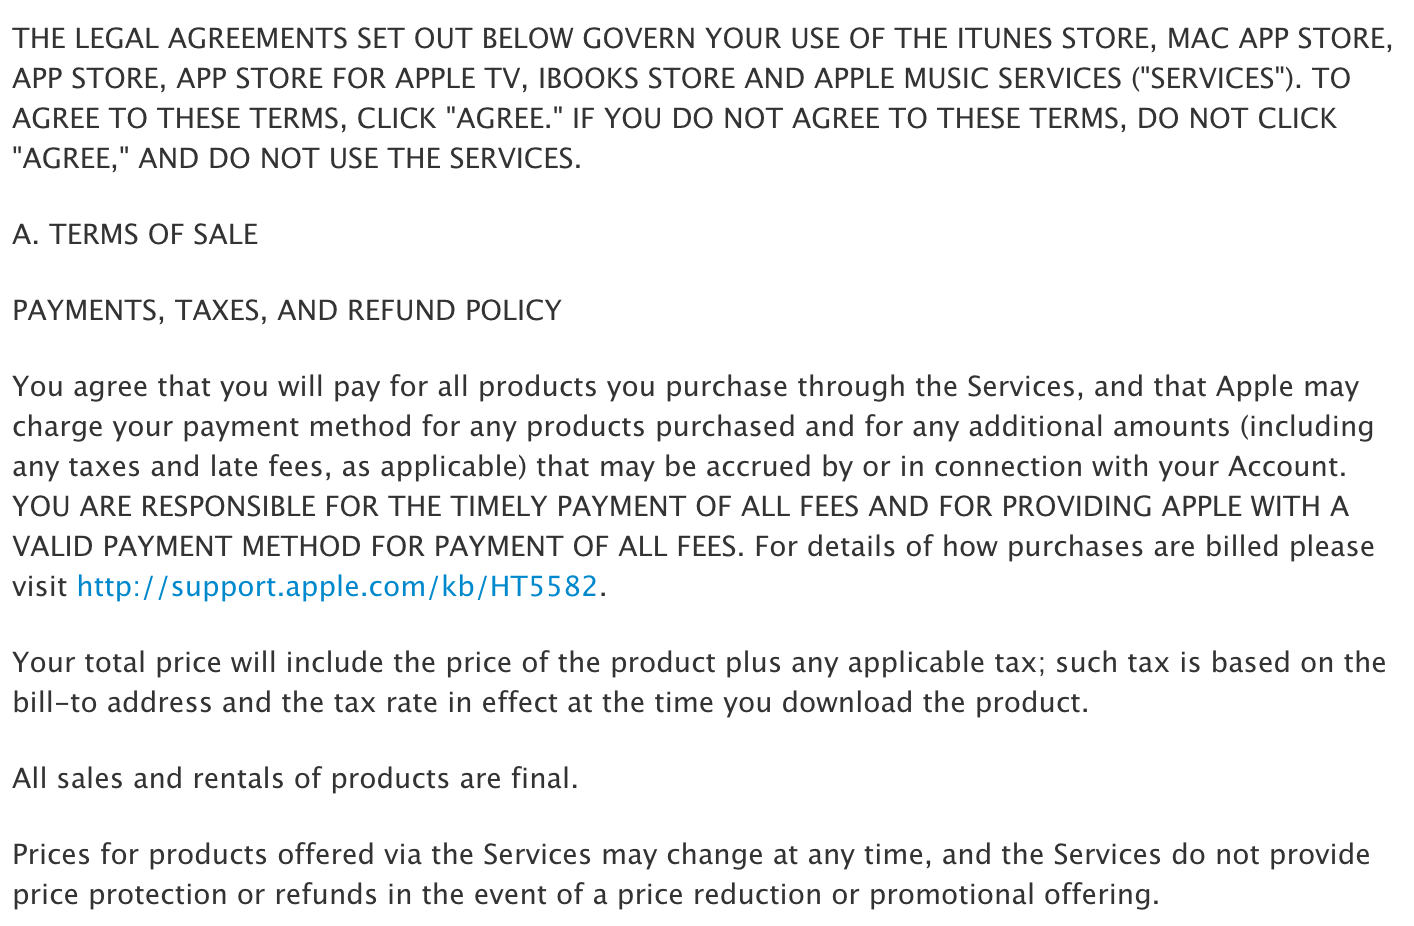
\includegraphics[totalheight=4cm]{legal_apple_ss.png}
      \caption{A sample text}
      \label{fig:verticalcell}
  \end{figure}

  Our training dataset contains 35 legal documents, which include 124,546 words. We use two documents for testing. One is the iTunes user agreement, which contains 1,329 words. We manually label some special sentences in this document. We then run our pipeline on this document, and use the number of labeled sentences highlighted by our pipeline as a measure of how successful the pipeline is. 

  The other document is the Atlassian's user agreement, which contains 7,934 words. Due to the size of this document, we cannot label all the sentences. Instead, we use this document for generalization test. We run our pipeline on Atalassian's user agreement, read the highlighted sentences, and subjectively check if these sentences are unordinary. Since the problem we defined is unsupervised, we can only evaluate the final results by subjective means. To increase the credibility of our evaluation, we also use quantitative methods for evaluating the robustness of our pipeline. We will discuss more about these methods in section 5. 

  We remove prepositions, numbers, punctuations because they add noise to our samples. For example, ``I have iphone'' and ``I have an iphone'' are treated as the same sentence in our pipeline. 

  % ; however the prepositional word would make these two sentences very different. Therefore, at the preprocessing stage we remove these noise words. 

  We also realize that some words with different suffixes may have the same meaning. For example, ``mature'' and ``maturity'' should be understood as the same word. In preprocessing step, we run an algorithm called \emph{Porter Stemming} \cite{porter} to convert words with the same stem and similar suffixes into one word. 

  We have two different sets of feature extraction and selection strategies. First, we use \emph{LDA} to construct common topic words across the training dataset. The feature extraction within \emph{LDA} is done by taking all documents as a single corpus and then by applying the variational inference method discussed in the original paper. 

  After running \emph{LDA} on all the documents, we get a list of topic words. A topic is a list of words, e.g. \emph{trademark, services, may, use, application, agreement, content}. We observe that these topic words do not contribute to the ``specialty '' of a sentence. Therefore, we remove the topic words from the test document.


  Second, for the test document, we use \emph{Word2Vec} to translate a word into a vector. \emph{Word2Vec} is a two-layer neural network. It takes text corpus as input and its output is a set of feature vectors for words in that corpus. For each word, we generate 100 features. These word vectors allow for numeric operations on words. For example, the vector of ``king'' added by the vector of ``woman'' would return the vector of ``queen''. After running \emph{Word2Vec}, we establish a mapping from words to vectors. 
  \begin{figure}[h!]
  \centering
          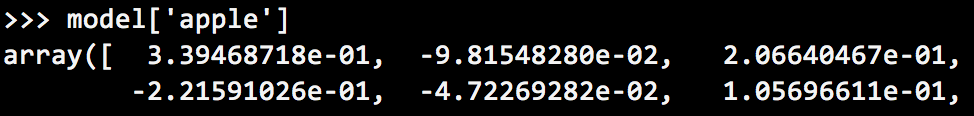
\includegraphics[height=0.7cm]{word2veceg3.png}
      \caption{Part of word vector of ``apple''}
      \label{fig:verticalcell}
  \end{figure}

  We assume that the feature vector of a sentence is the sum of feature vectors of all the words in this sentence. We then run clustering algorithms on the vector representations of all the sentences. 

\section{Methods}
  We use \emph{EM} algorithm to learn the hidden parameters of the \emph{LDA} model. We then use \emph{Agglomerative Clustering} and \emph{LOF} to learn the distributions of unordinary sentences in the document. We will discuss these methods in the following subsections. 

  \subsection{\emph{EM} for estimating \emph{LDA} parameters}
  The \emph{LDA} model uses a word \emph{w} as a basic unit. A document is a sequence of $N$ words denoted by $\textbf{w} = (w_1, \cdots, w_N )$. A corpus contains $M$ documents is denoted by $\textbf{D} = \{ \textbf{w}_1, \cdots, \textbf{w}_M \}$.  

  \emph{LDA} takes the following generative steps for each document \textbf{w} in a corpus \textbf{D}:

\begin{enumerate}

    \item Choose $N$ $\sim$ Poisson($\xi$).
    \item Choose $\theta$ $\sim$ Dir($\alpha$).
    \item For each of the $N$ words $\textbf{w}_n$:
    \begin{enumerate}[label=\roman*]
      \item Choose a topic $z_n \sim$ Multinomial($\theta$).
      \item Choose a word $w_n$ from $p(w_n | z_n, \beta)$, where $p$ is a multinomial probability conditioned on $z_n$ and $\beta$. 
    \end{enumerate}
\end{enumerate}
  
  The probability of seeing an $N$ word document, $P(\textbf{w}|\alpha, \beta)$, is given as: 

  $P(\textbf{w}|\alpha, \beta) = \int(\Pi_{n=1}^N \sum_z P(w_n | z, \beta) P(z | \theta))  P(\theta | \alpha) d \theta$. \\

  To estimate the two hidden parameters, $(\alpha, \beta)$, from a corpus \textbf{D}, one needs to maximize the log likelihood: 

  $\log P(\textbf{D} | \alpha, \beta) = \sum_{d=1}^M \log P(\textbf{w}^{(d)} | \alpha, \beta)$, \\
  which is not tractable. To resolve this issue, the $LDA$ paper recommends to use variational inference method. The key of this method is to apply \emph{Jensen's Inequality} to obtain a lower bound of $\log P(\textbf{w} | \alpha, \beta)$. Let $q(z, \theta)$ be the joint pdf of $z, \theta$. Then: 

  $\log P(\textbf{w} | \alpha, \beta) \geq \int \sum_z q(z,\theta) \log \frac{P(\textbf{w}, z, \theta | \alpha, \beta)}{q(z, \theta)} d\theta$

  $ = L(\alpha, \beta)$. \\
  Note that: 

  $L(\alpha, \beta) = \int \sum_z q(z, \theta) \log \frac{P(\textbf{w}, z, \theta | \alpha, \beta)}{q(z, \theta)} d\theta$

  $ = \int \sum_z q(z, \theta) (\log \frac{P(z, \theta | \textbf{w}, \alpha, \beta)}{q(z, \theta)} + \log P(\textbf{w} | \alpha, \beta)) d\theta$

  $ = - \int \sum_z q(z, \theta) \log \frac{q(z,\theta)}{P(z, \theta; \textbf{w}, \alpha, \beta)} d \theta $ 

  $+ \int \sum_z q (z, \theta) \log P(\textbf{w} | \alpha, \beta) d \theta$

  $ = -KL(q(z,\theta) || P(z, \theta | \textbf{w}, \alpha, \beta)) + \log P(\textbf{w} | \alpha, \beta)$

  $ \leftrightarrow \log P(\textbf{w} | \alpha, \beta) = L(\alpha, \beta) + KL(q(z,\theta) || P(z, \theta | \textbf{w}, \alpha, \beta))$. \\
  Since we want to find a $L(\alpha, \beta)$ that is as much close to $\log P(\textbf{w} | \alpha, \beta)$ as possible, we want to find a parameterized $q(z, \theta)$ that has as small KL-distance to $q(z, \theta)$ as possible. 

  Let $z, \theta$ be parameterized by $\phi, \gamma$ respectively, 

  i.e.: $q(z, \theta) = q(\theta | \gamma) \Pi_{n=1}^N q(z_n | \phi^{(n)})$. \\
  Let $L(\phi, \gamma; \alpha, \beta)$ denotes the lower-bound of $\log P(\textbf{w} | \alpha, \beta)$. Then: 

  $\log P(\textbf{D} | \alpha, \beta) \geq \sum_{d=1}^M L(\textbf{w}^{(d)}; \phi^{(1,d), \cdots, \phi^{N_d, d}}, \gamma^{(d)}; \alpha, \beta) $


  = \textbf{L} $(\Phi, \Gamma; \alpha, \beta)$, \\
  where $\Phi = [\phi^{(n,d)}], \Gamma = [\gamma^{(d)}]$. \\

  The idea of $EM$ is to start from initial $\alpha, \beta$, and iteratively improve the estimate: \\
  \emph{E-step}: Given $\alpha, \beta$,

   $(\Phi, \Gamma) := \arg \max_{(\Phi, \Gamma)} \textbf{L}(\Phi, \Gamma; \alpha, \beta)$; \\
   \emph{M-step}: Given $\Phi, \Gamma$, 

   $(\alpha, \beta) := \arg \max_{(\alpha, \beta)} \textbf{L}(\Phi, \Gamma; \alpha, \beta)$.

   These two steps are repeated until \textbf{L} converges. We won't show the complete derivation here, but we use the following updating equations for getting $(\alpha, \beta)$. \\
  In \emph{E-step}, the update equations for $\Phi$ and $\Gamma$ are: 

  $\phi_i^{(n,d)} :\propto \beta_{i, w_n^{(d)}} \exp (\digamma (\gamma_i^{(d)}) - \digamma(\sum_j \gamma_j^{(d)}))$ \\
  where $\digamma$ is the digamma function; 

  $\gamma_i^{(d)} := \alpha_i + \sum_{n=1}^{N_d} \phi_i^{(n,d)}$. \\
  In \emph{M-step}, the update equation for $\beta$ is: 

  $\beta_{ij} :\propto \sum_{d=1}^M \sum_{n=1}^{N_d} \phi_i^{(n,d)} \textbf{1}(w_n^{d} = j)$. \\
  There is no analytical solution to $\alpha$, but it can be obtained by maximizing

  $L_\alpha = \sum_d (\log \bar{\Gamma} (\sum_{i=1}^K \alpha_i)  - \sum_{i=1}^K \log \bar{\Gamma} (\alpha_i) $

  $ + \sum_{i=1}^K (\alpha_i -1)(\digamma(\gamma_i^{(d)}) - \digamma(\sum_{j=1}^K \gamma_j^{(d)})))$ \\
  using Newton's method, where $\bar{\Gamma}$ is the gamma function. 

  \subsection{Agglomerative Clustering}
  For a new test document, we first get the feature vector of each sentence. We then use \emph{Agglomerative Clustering} to segment the document. We first specify that we want to have $N$ clusters. We then put each sentence into its own cluster, and iteratively merge the closest clusters until only $N$ clusters remain. We then look at these clusters. If there exists a cluster that contains only one sentence, then we know that this sentence is a special one, as it is never merged into other clusters. 

  We define the cosine similarity between two sentences as the dot product of their normalized vector representations. We then calculate cosine distance from cosine similarity and use this distance as our clustering metric. 

  The distance between any two clusters $A$ and $B$ is taken to be the mean distance between elements of each cluster \cite{upgma}. 

  In section $5$, we will discuss on how to choose the right number of clusters to achieve the best clustering structure. 

  It is worth mentioning that we find \emph{K-means} and \emph{K-means++} performing much more unstable than \emph{Agglomerative Clustering} in our case. The final outcome of \emph{K-means} and \emph{K-means++} depends heavily on the initial assignments of the centroids. However, since both methods choose initial centroids in a semi-random fashion, it is not guaranteed that the final clustering would remain the same from run to run. In contrast, \emph{Agglomerative Clustering} does not depend on initial assignments. As a result, it creates more stable outcomes. 

  Before running \emph{LOF}, we recommend to run \emph{Agglomerative Clustering} first, and then remove the discovered anormaly sentences from the test document. The reason is that we want to decrease the local density around unordinary sentences so that these sentences can be more easily picked up by \emph{LOF}. 


  % Find local 
  \subsection{Local Outlier Factor (LOF)}
  In our feature space, each sentence is represented as a point. Therefore, if we find a point with low local density, then this point is an outlier, and its corresponding sentence is unordinary. 

  To help explain how \emph{LOF} works, we introduce two terms:

  $\text{N}_k(A)$: Set of $k$ nearest neighbors to $A$. 

  k-D($A$): distance from $A$ to its $k^{th}$ nearest neighbor. 

  $\text{RD}_k (A,B) = \max \{ \text{k-D} (A,B), \text{distance}(A,B) \}$, where $RD$ denotes reachability distance. We use the maximum of two distances to get a stable result. \\

  The local reachability density of $A$ is computed as: 

  $\text{lrd}(A) = 1 / (\frac{\sum_{B\in \text{N}_k(A)} \text{RD}_k(A,B)}{|\text{N}_k(A)|})$. \\
  It is then compared with its neighbors using: 

  $LOF_k(A) = \frac{\sum_{B \in \text{N}_k(A)} \text{lrd}(B) }{|\text{N}_k(A)|} / \text{lrd}(A)$, \\
  which is the average local density of neighbors divided by the object's own local density. If this value is greater than $1$, it tells that the local density around this object is lower than its neighbors, and thus is an outlier. 

  This method studies the local distribution of points, and helps us improve the performance on top of \emph{Agglomerative Clustering}. Basically, it is hard to have insight of how points are distributed within an agglomerative cluster. Using \emph{LOF} helps us understand the distribution of points within a cluster. 

\section{Experiments and Results}
  In this section, we first discuss how we choose the hyperparameters for \emph{LDA} and for \emph{Agglomerative Clustering}. We will then talk about the performance achieved by our pipeline on the test cases.

  \subsection{Tuning Hyperparameters}
  In this subsection, we will use the iTunes user agreement as an example to show how our hyperparameter choosing strategy works. There are 42 sentences and 1329 words in this document. 

  \subsubsection{Choosing parameter for \emph{LDA} model}
  For \emph{LDA} model, number of topics is a critical parameter. We enumerate over possible number of topics and study how the perplexity changes. We then use the number of topics that yields the best perplexity. 

  Documents in our training dataset are unlabeled. Therefore, we wish to achieve high likelihood on a held-out testset. In fact, we use the perplexity of a held-out test set to evaluate the model. 

  Intuitively, a lower perplexity score indicates better generalization performance. The perplexity is equivalent to the inverse of the geometric mean per-word likelihood: 

  $perplexity(D_{\text{test}}) = \exp( - \frac{\sum_{d=1}^M \log p(w_d)}{\sum_{d=1}^M N_d})$, \\
   using the same notation as in section 4.1. 

  In our experiment, we use the corpus generated by parsing html pages of legal documents from Atlassian, Github, and Apple. We held out 25\% of the data and trained on the remaining 75\%. 
  \begin{figure}[h!]
  \centering
          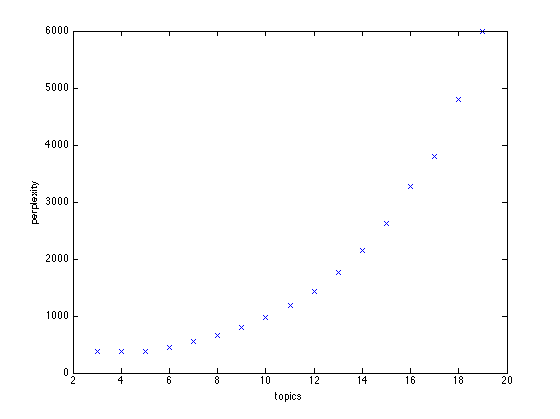
\includegraphics[height=4cm]{perplexity.png}
      \caption{perplexity given number of topics}
      \label{fig:verticalcell}
  \end{figure}

  We found that the perplexity is the lowest when there are around 3 $\sim$ 5 topics. We found that for the iTunes user agreement, using 5 topics works the best for improving the differences between sentences. 

  \subsubsection{Choosing number of clusters}
  We use \emph{Silhouettes} \cite{sil} score to evaluate the robustness of clusters. We enumerate over possible numbers of clusters, and pick the one that yields the best \emph{Silhouettes} score. 

  Intuitively, larger \emph{Silhouettes} score indicates that the distance between each cluster is large, and the maximum distance from the farthest point in a cluster to its centroid is small. The formal definition is given as follows: 

  For each point $i$, let $a(i)$ be the average dissimilarity of $i$ with all other points in the same cluster. Let $b(i)$ be the lowest average dissimilarity of $i$ to any other cluster, of which $i$ does not belong to. The cluster with the lowest average dissimilarity is defined to be the neighboring cluster of $i$. This cluster is also the next best fit for $i$. \emph{Silhouettes} score is defined as: 

  $s(i) = \frac{b(i) - a(i)}{\max\{a(i), b(i)\}} $, where $-1 \leq s(i) \leq 1$. \\

  If $s(i)$ is close to 1, it means that the average dissimilarity between $i$ and its neighboring cluster is much greater than the dissimialrity between $i$ and its own cluster. In this case, we say that $i$ is properly clustered. In contrast, if $s(i)$ is close to -1, it means that $i$ would be more properly labeled by its neighboring cluster. We use the average of $s(i)$ over all sentence vectors of the test document as a measure of how tight each cluster is and how far away each cluster is from its neighbors. The curve is shown in figure 4. 

  \begin{figure}[h!]
  \centering
          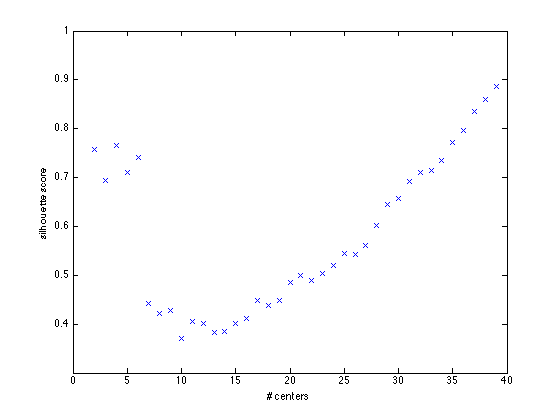
\includegraphics[height=4cm]{sildis.png}
      \caption{Silhouette score given number of centroids}
      \label{fig:verticalcell}
  \end{figure}  

  From figure 4, the average \emph{Silhouettes} score is high when more than 27 clusters are used. The reason is that when having more than 27 clusters, most of these clusters contain only one sentence from the iTunes user agreement. As a result, the average dissimilarity within each of these clusters is 0, and the corresponding \emph{Silhouettes} score goes up to 1. 

  In practice, we do not use more than 27 clusters. The major concern is that if most of the clusters contain only one sentence, then we cannot tell if this sentence is an anormaly or not. Therefore, we only look at the \emph{Silhouettes} scores when we have few clusters, and we find that having 3 clusters works the best. 

  \subsection{Visualization}
  In this subsection, we look at how the unordinary sentences picked up by our pipeline distribute in 3D space. We use \emph{t-SNE} \cite{tsne} and \emph{PCA} to extract three dimensions from features of our results. In both figures, points in dim yellow or blue are farther from the view point. The blue triangles mark positions of unordinary sentences. 

  \begin{figure}[h!]
  \centering
          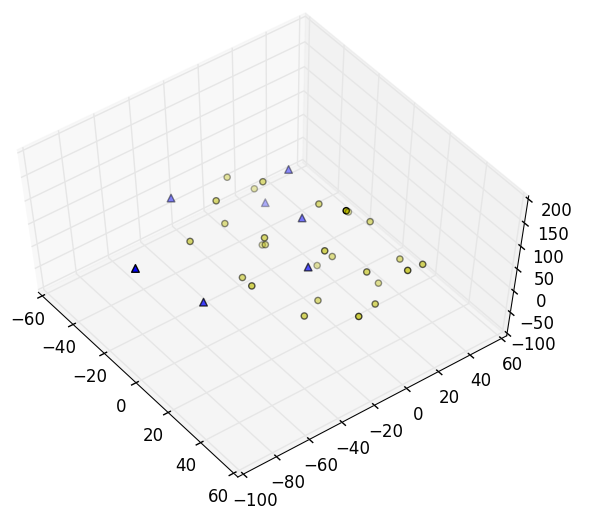
\includegraphics[height=4cm]{tsne_report.png}
      \caption{first 3 dimensions of \emph{t-SNE} result}
      \label{fig:verticalcell}
  \end{figure}  

  In figure 5, as we can see, the unordinary sentences locate at places with lower local density. 

  \begin{figure}[h!]
  \centering
          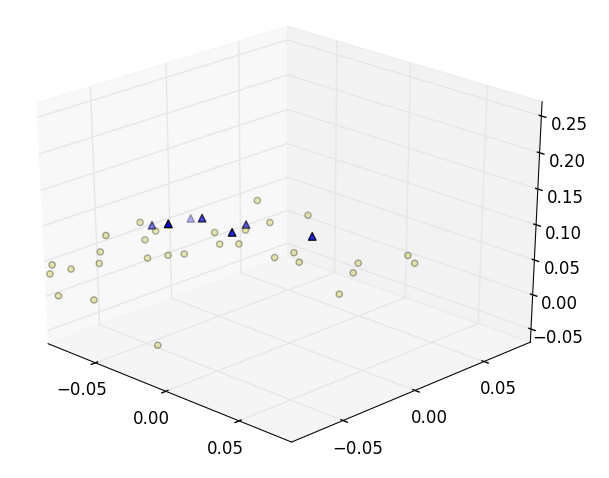
\includegraphics[height=4cm]{PCA_result.png}
      \caption{first 3 dimensions of \emph{PCA} result}
      \label{fig:verticalcell}
  \end{figure}  

  In figure 6, result of PCA also shows that unordinary sentences are picked up at locations with lower local densities. However, in figure 6, points are denser than in figure 5. This indicates that \emph{t-SNE} does a better job on signifying the differences between points than \emph{PCA} does. 

  \subsection{Tests}
  Since we are trying to solve an unsupervised learning problem, it is hard to quantify test accuracy. To mitigate that, we create test cases by using three groups of sentences:
  \begin{enumerate}
    \item We insert irrelevant sentences into the test document. For example, we added ``we are such stuff as dreams are made on our little life is rounded with sleep'', which is a quote from Shakespeare. 

    \item We modify original text. For example, we change ``apple reserves the right ...'' to ``Apple reserves ... to be scrutinized by great fire wall of China''.

    \item We subjectively choose some special sentences. For example, we highlight ``you further agree to not... harassing, threatening, defamatory ...'' as a special sentence. 
  \end{enumerate}

  For iTunes EULA (small test case), we inserted 3 totally irrelevant sentences, modified 7 original sentences, and subjectively chose 10 special sentences. 

  For Atlassian's EULA (large test case), we inserted 3 totally irrelevant sentences, modified 10 orignal sentences, and subjectively chose 10 special sentences. 

  We choose to not insert or modify a lot of sentences within the test documents. The reason is that as the number of modified or inserted sentences increases, the chance of randomly picking one sentence and observing that the sentence is in Group 1 or 2 also increases. Thus, inserting and modifying few sentences in the large test document help to show that our pipeline does not succeed by choosing sentences randomly. 

  We run our pipeline on these test cases , and we check how many of sentences in each group are picked up by our pipeline. The result is shown in the following table: 

\begin{center}
  \begin{tabular}{ | l || c || c ||}
    \hline
                & iTunes' EULA & Atlassian's EULA \\ \hline
     \# of words       & 1329    & 7934 \\ \hline
     \# of sentences   & 42      & 282  \\ \hline
     \% of Group 1 & 100  \% & 100 \% \\ \hline
     \% of Group 2 & 28.5 \% & 10 \% \\ \hline % 2/7, 1/10
     \% of Group 3 & 60 \% & 40 \% \\ \hline % 
  \end{tabular}
\end{center}

  From the table, it is shown that our pipeline is very accurate on picking up irrelevant sentences. However, it does poorly on picking up partially modified sentences. We find out that our assumption on generating the sentence vector causes this problem, and we will discuss possible improvements in section 6. It seems that our pipeline does not perform well on picking up Group 3 sentences. The reason is that when manually creating test cases, it is very hard for us to pick up all the unordinary sentences. Moreover, we sometimes pick up sentences that are actually quite common in legal documents due to our limited knowledge of how user agreements are written.

  Therefore, to better evaluate the performance on Group 3 sentences, we read the output from our pipeline, and manually construct a confusion matrix for it. For the large test case: 

  \begin{center}
    \begin{tabular}{|| c || c ||}
      \hline
         true positives: 10 & false positives: 2 \\ \hline
         false negatives: N/A & true negatives: N/A \\ \hline % 
    \end{tabular}
  \end{center}

  We cannot give an account on false negatives and true negatives, because for a lot of sentences we cannot confidently tell if it is too ordinary. 

  \section{Future Work}
  In this report, we propose a pipeline that finds unordinary sentences in a given legal document. We construct the pipeline by first building a training dataset of many legal documents sharing similar topics. We then use \emph{LDA} model with \emph{EM} algorithm to find the common topic words across the dataset. When coming to a new test document, we first remove common topic words from it to increase differences between sentences. We then use \emph{Word2Vec} to extract sentence features, cluster the sentences and use \emph{LOF} to find the outliers. Finally, we run \emph{t-SNE} and \emph{PCA} to visualize the first 3 dimensions of the result. 

  We evaluate the performance of our pipeline using two types of method. First, we check perplexity of the \emph{LDA} model and \emph{Silhouettes} score of the clusters to measure the robustness of our model. Second, we manually create test cases by adding three groups of sentences, and we measure the performance of our pipeline on these test cases. 

  Regarding finding unordinary sentences, the majority of the job is done by \emph{LOF}. This is because most of the sentences use similar words and are clustered closely. As a result, clustering cannot filter out a lot of unordinary sentences. However, \emph{LOF} only considers the local density of an area regardless of which cluster it belongs to. As a result, \emph{LOF} is able to pick up more differences between sentences. 

  Future work includes improving our sentence model. Meanwhile, we make a naive assumption that the vector of a sentence is the sum of vectors of words. However, this assumption ignores the semantics of phrases in a sentence. Therefore, the next step of improvement would be to consider more of relation between words within a sentence. For example, we can use a bigram or trigram model to address the correlation between words in a sentence. 

  % There is no analytical solution to $\alpha$, but it can be achieved by maximizing the following target function using Newton's method: 

  % $( , \textbf{\gamma}; \textbf{\alpha}, \textbf{\beta} )$

% An example of a floating figure using the graphicx package.
% Note that \label must occur AFTER (or within) \caption.
% For figures, \caption should occur after the \includegraphics.
% Note that IEEEtran v1.7 and later has special internal code that
% is designed to preserve the operation of \label within \caption
% even when the captionsoff option is in effect. However, because
% of issues like this, it may be the safest practice to put all your
% \label just after \caption rather than within \caption{}.
%
% Reminder: the "draftcls" or "draftclsnofoot", not "draft", class
% option should be used if it is desired that the figures are to be
% displayed while in draft mode.
%
%\begin{figure}[!t]
%\centering
%\includegraphics[width=2.5in]{myfigure}
% where an .eps filename suffix will be assumed under latex, 
% and a .pdf suffix will be assumed for pdflatex; or what has been declared
% via \DeclareGraphicsExtensions.
%\caption{Simulation results for the network.}
%\label{fig_sim}
%\end{figure}

% Note that the IEEE typically puts floats only at the top, even when this
% results in a large percentage of a column being occupied by floats.


% An example of a double column floating figure using two subfigures.
% (The subfig.sty package must be loaded for this to work.)
% The subfigure \label commands are set within each subfloat command,
% and the \label for the overall figure must come after \caption.
% \hfil is used as a separator to get equal spacing.
% Watch out that the combined width of all the subfigures on a 
% line do not exceed the text width or a line break will occur.
%
%\begin{figure*}[!t]
%\centering
%\subfloat[Case I]{\includegraphics[width=2.5in]{box}%
%\label{fig_first_case}}
%\hfil
%\subfloat[Case II]{\includegraphics[width=2.5in]{box}%
%\label{fig_second_case}}
%\caption{Simulation results for the network.}
%\label{fig_sim}
%\end{figure*}
%
% Note that often IEEE papers with subfigures do not employ subfigure
% captions (using the optional argument to \subfloat[]), but instead will
% reference/describe all of them (a), (b), etc., within the main caption.
% Be aware that for subfig.sty to generate the (a), (b), etc., subfigure
% labels, the optional argument to \subfloat must be present. If a
% subcaption is not desired, just leave its contents blank,
% e.g., \subfloat[].


% An example of a floating table. Note that, for IEEE style tables, the
% \caption command should come BEFORE the table and, given that table
% captions serve much like titles, are usually capitalized except for words
% such as a, an, and, as, at, but, by, for, in, nor, of, on, or, the, to
% and up, which are usually not capitalized unless they are the first or
% last word of the caption. Table text will default to \footnotesize as
% the IEEE normally uses this smaller font for tables.
% The \label must come after \caption as always.
%
%\begin{table}[!t]
%% increase table row spacing, adjust to taste
%\renewcommand{\arraystretch}{1.3}
% if using array.sty, it might be a good idea to tweak the value of
% \extrarowheight as needed to properly center the text within the cells
%\caption{An Example of a Table}
%\label{table_example}
%\centering
%% Some packages, such as MDW tools, offer better commands for making tables
%% than the plain LaTeX2e tabular which is used here.
%\begin{tabular}{|c||c|}
%\hline
%One & Two\\
%\hline
%Three & Four\\
%\hline
%\end{tabular}
%\end{table}


% Note that the IEEE does not put floats in the very first column
% - or typically anywhere on the first page for that matter. Also,
% in-text middle ("here") positioning is typically not used, but it
% is allowed and encouraged for Computer Society conferences (but
% not Computer Society journals). Most IEEE journals/conferences use
% top floats exclusively. 
% Note that, LaTeX2e, unlike IEEE journals/conferences, places
% footnotes above bottom floats. This can be corrected via the
% \fnbelowfloat command of the stfloats package.




% conference papers do not normally have an appendix



% use section* for acknowledgment
\ifCLASSOPTIONcompsoc
  % The Computer Society usually uses the plural form
  \section*{Acknowledgments}
\else
  % regular IEEE prefers the singular form
  \section*{Acknowledgment}
\fi


We would like to thank CS229 staff for their help through the quarter.

We would like to thank Albert Haque, our project mentor, for his great ideas that help us improve the project. 

We would also like to thank Prof. Andrew Ng for the great class. 



% trigger a \newpage just before the given reference
% number - used to balance the columns on the last page
% adjust value as needed - may need to be readjusted if
% the document is modified later
%\IEEEtriggeratref{8}
% The "triggered" command can be changed if desired:
%\IEEEtriggercmd{\enlargethispage{-5in}}

% references section

% can use a bibliography generated by BibTeX as a .bbl file
% BibTeX documentation can be easily obtained at:
% http://mirror.ctan.org/biblio/bibtex/contrib/doc/
% The IEEEtran BibTeX style support page is at:
% http://www.michaelshell.org/tex/ieeetran/bibtex/
%\bibliographystyle{IEEEtran}
% argument is your BibTeX string definitions and bibliography database(s)
%\bibliography{IEEEabrv,../bib/paper}
%
% <OR> manually copy in the resultant .bbl file
% set second argument of \begin to the number of references
% (used to reserve space for the reference number labels box)
\newpage
\begin{thebibliography}{1}

\bibitem{lda}
Blei, David M., Andrew Y. Ng, and Michael I. Jordan. ``Latent dirichlet allocation.'' the Journal of machine Learning research 3 (2003): 993-1022.

\bibitem{one}
Mikolov, Tomas, et al. ``Efficient estimation of word representations in vector space.'' arXiv preprint arXiv:1301.3781 (2013).

\bibitem{two}
Mikolov, Tomas, et al. ``Distributed representations of words and phrases and their compositionality.'' Advances in neural information processing systems. 2013.


\bibitem{lof}
Breunig, Markus M., et al. ``LOF: identifying density-based local outliers.'' ACM sigmod record. Vol. 29. No. 2. ACM, 2000.

\bibitem{tsne}
Van der Maaten, Laurens, and Geoffrey Hinton. ``Visualizing data using t-SNE.'' Journal of Machine Learning Research 9.2579-2605 (2008): 85.

\bibitem{three}
Radim Rehurek, \href{https://radimrehurek.com/gensim/models/word2vec.html#id4}{\emph{Optimizing word2vec in gensim}}. Nov 07, 2015

\bibitem{reviewcite1}
Qazvinian, Vahed, and Dragomir R. Radev. ``Scientific paper summarization using citation summary networks.'' Proceedings of the 22nd International Conference on Computational Linguistics-Volume 1. Association for Computational Linguistics, 2008.

\bibitem{reviewcite2}
Cai, Xiaoyan, et al. ``Simultaneous ranking and clustering of sentences: a reinforcement approach to multi-document summarization.''  Proceedings of the 23rd International Conference on Computational Linguistics. Association for Computational Linguistics, 2010.

\bibitem{reviewcite3}
Nanba, Hidetsugu, and Manabu Okumura. ``Towards multi-paper summarization using reference information.'' IJCAI. Vol. 99. 1999.

\bibitem{reviewcite4}
Mahapatra, Amogh, Nisheeth Srivastava, and Jaideep Srivastava. ``Contextual anomaly detection in text data.'' Algorithms 5.4 (2012): 469-489.

\bibitem{porter}
Porter, Martin. ``The Porter stemming algorithm, 2005.'' See http://www.tartarus.org/$\sim$martin/PorterStemmer.

\bibitem{upgma}
Sokal, Robert R. ``A statistical method for evaluating systematic relationships.'' Univ Kans Sci Bull 38 (1958): 1409-1438.

\bibitem{sil}
Rousseeuw, Peter J. ``Silhouettes: a graphical aid to the interpretation and validation of cluster analysis.'' Journal of computational and applied mathematics 20 (1987): 53-65.

\end{thebibliography}





% that's all folks
\end{document}


